%Notes by Harsh Mistry 
%CS 350
%Based on Template From  https://www.cs.cmu.edu/~ggordon/10725-F12/template.tex

\documentclass[twoside]{article}
\setlength{\oddsidemargin}{0.25 in}
\setlength{\evensidemargin}{-0.25 in}
\setlength{\topmargin}{-0.6 in}
\setlength{\textwidth}{6.5 in}
\setlength{\textheight}{8.5 in}
\setlength{\headsep}{0.75 in}
\setlength{\parindent}{0 in}
\setlength{\parskip}{0.1 in}
\usepackage{amsmath,amsfonts,graphicx}
\newcounter{lecnum}
\renewcommand{\thepage}{\thelecnum-\arabic{page}}
\renewcommand{\thesection}{\thelecnum.\arabic{section}}
\renewcommand{\theequation}{\thelecnum.\arabic{equation}}
\renewcommand{\thefigure}{\thelecnum.\arabic{figure}}
\renewcommand{\thetable}{\thelecnum.\arabic{table}}
\newcommand{\lecture}[4]{
   \pagestyle{myheadings}
   \thispagestyle{plain}
   \newpage
   \setcounter{lecnum}{#1}
   \setcounter{page}{1}
   
   \graphicspath{ {images/} }
   
%Info Box 
   \begin{center}
   \framebox{
      \vbox{\vspace{2mm}
    \hbox to 6.28in { {\bf CS 350 - Operating Systems
	\hfill Winter 2018} }
       \vspace{4mm}
       \hbox to 6.28in { {\Large \hfill Lecture #1: #2  \hfill} }
       \vspace{2mm}
       \hbox to 6.28in { {\it Lecturer: #3 \hfill Notes By: #4} }
      \vspace{2mm}}
   }
   \end{center}
   
   \markboth{Lecture #1: #2}{Lecture #1: #2}



 
}

\renewcommand{\cite}[1]{[#1]}
\def\beginrefs{\begin{list}%
        {[\arabic{equation}]}{\usecounter{equation}
         \setlength{\leftmargin}{2.0truecm}\setlength{\labelsep}{0.4truecm}%
         \setlength{\labelwidth}{1.6truecm}}}
\def\endrefs{\end{list}}
\def\bibentry#1{\item[\hbox{[#1]}]}

\newcommand{\fig}[3]{
			\vspace{#2}
			\begin{center}
			Figure \thelecnum.#1:~#3
			\end{center}
	}

\newtheorem{theorem}{Theorem}[lecnum]
\newtheorem{lemma}[theorem]{Lemma}
\newtheorem{ex}[theorem]{Example}
\newtheorem{proposition}[theorem]{Proposition}
\newtheorem{claim}[theorem]{Claim}
\newtheorem{corollary}[theorem]{Corollary}
\newtheorem{definition}[theorem]{Definition}
\newenvironment{proof}{{\bf Proof:}}{\hfill\rule{2mm}{2mm}}
\newcommand\E{\mathbb{E}}


%Start of Document 
\begin{document}

\lecture{2}{January 8, 2018}{Lesley Istead}{Harsh Mistry}

\section{Threads and Concurrency}

\textbf{What is a Thread?}
\begin{itemize}
\item Threads provide a way for programmers to express \textbf{concurrency} in a program
\item A normal \textbf{sequential program consist of single thread of execution}
\item In threaded concurrent programs there are multiple threads of execution, all occurring at the same time.
\end{itemize}

\textbf{Key Ideas}
\begin{itemize}
\item A thread can create new threads using \verb|thread_fork|
\item New threads can start execution in a function specified as a parmeter to \verb|thread_fork|
\item The original thread proceed concurrently, as two simultaneous sequential threads of execution
\item All threads share access to the program's global variables and heap
\item Each thread's function activations are private to the thread. 
\end{itemize}

\textbf{OS/161 Thread Interface}
\begin{center}
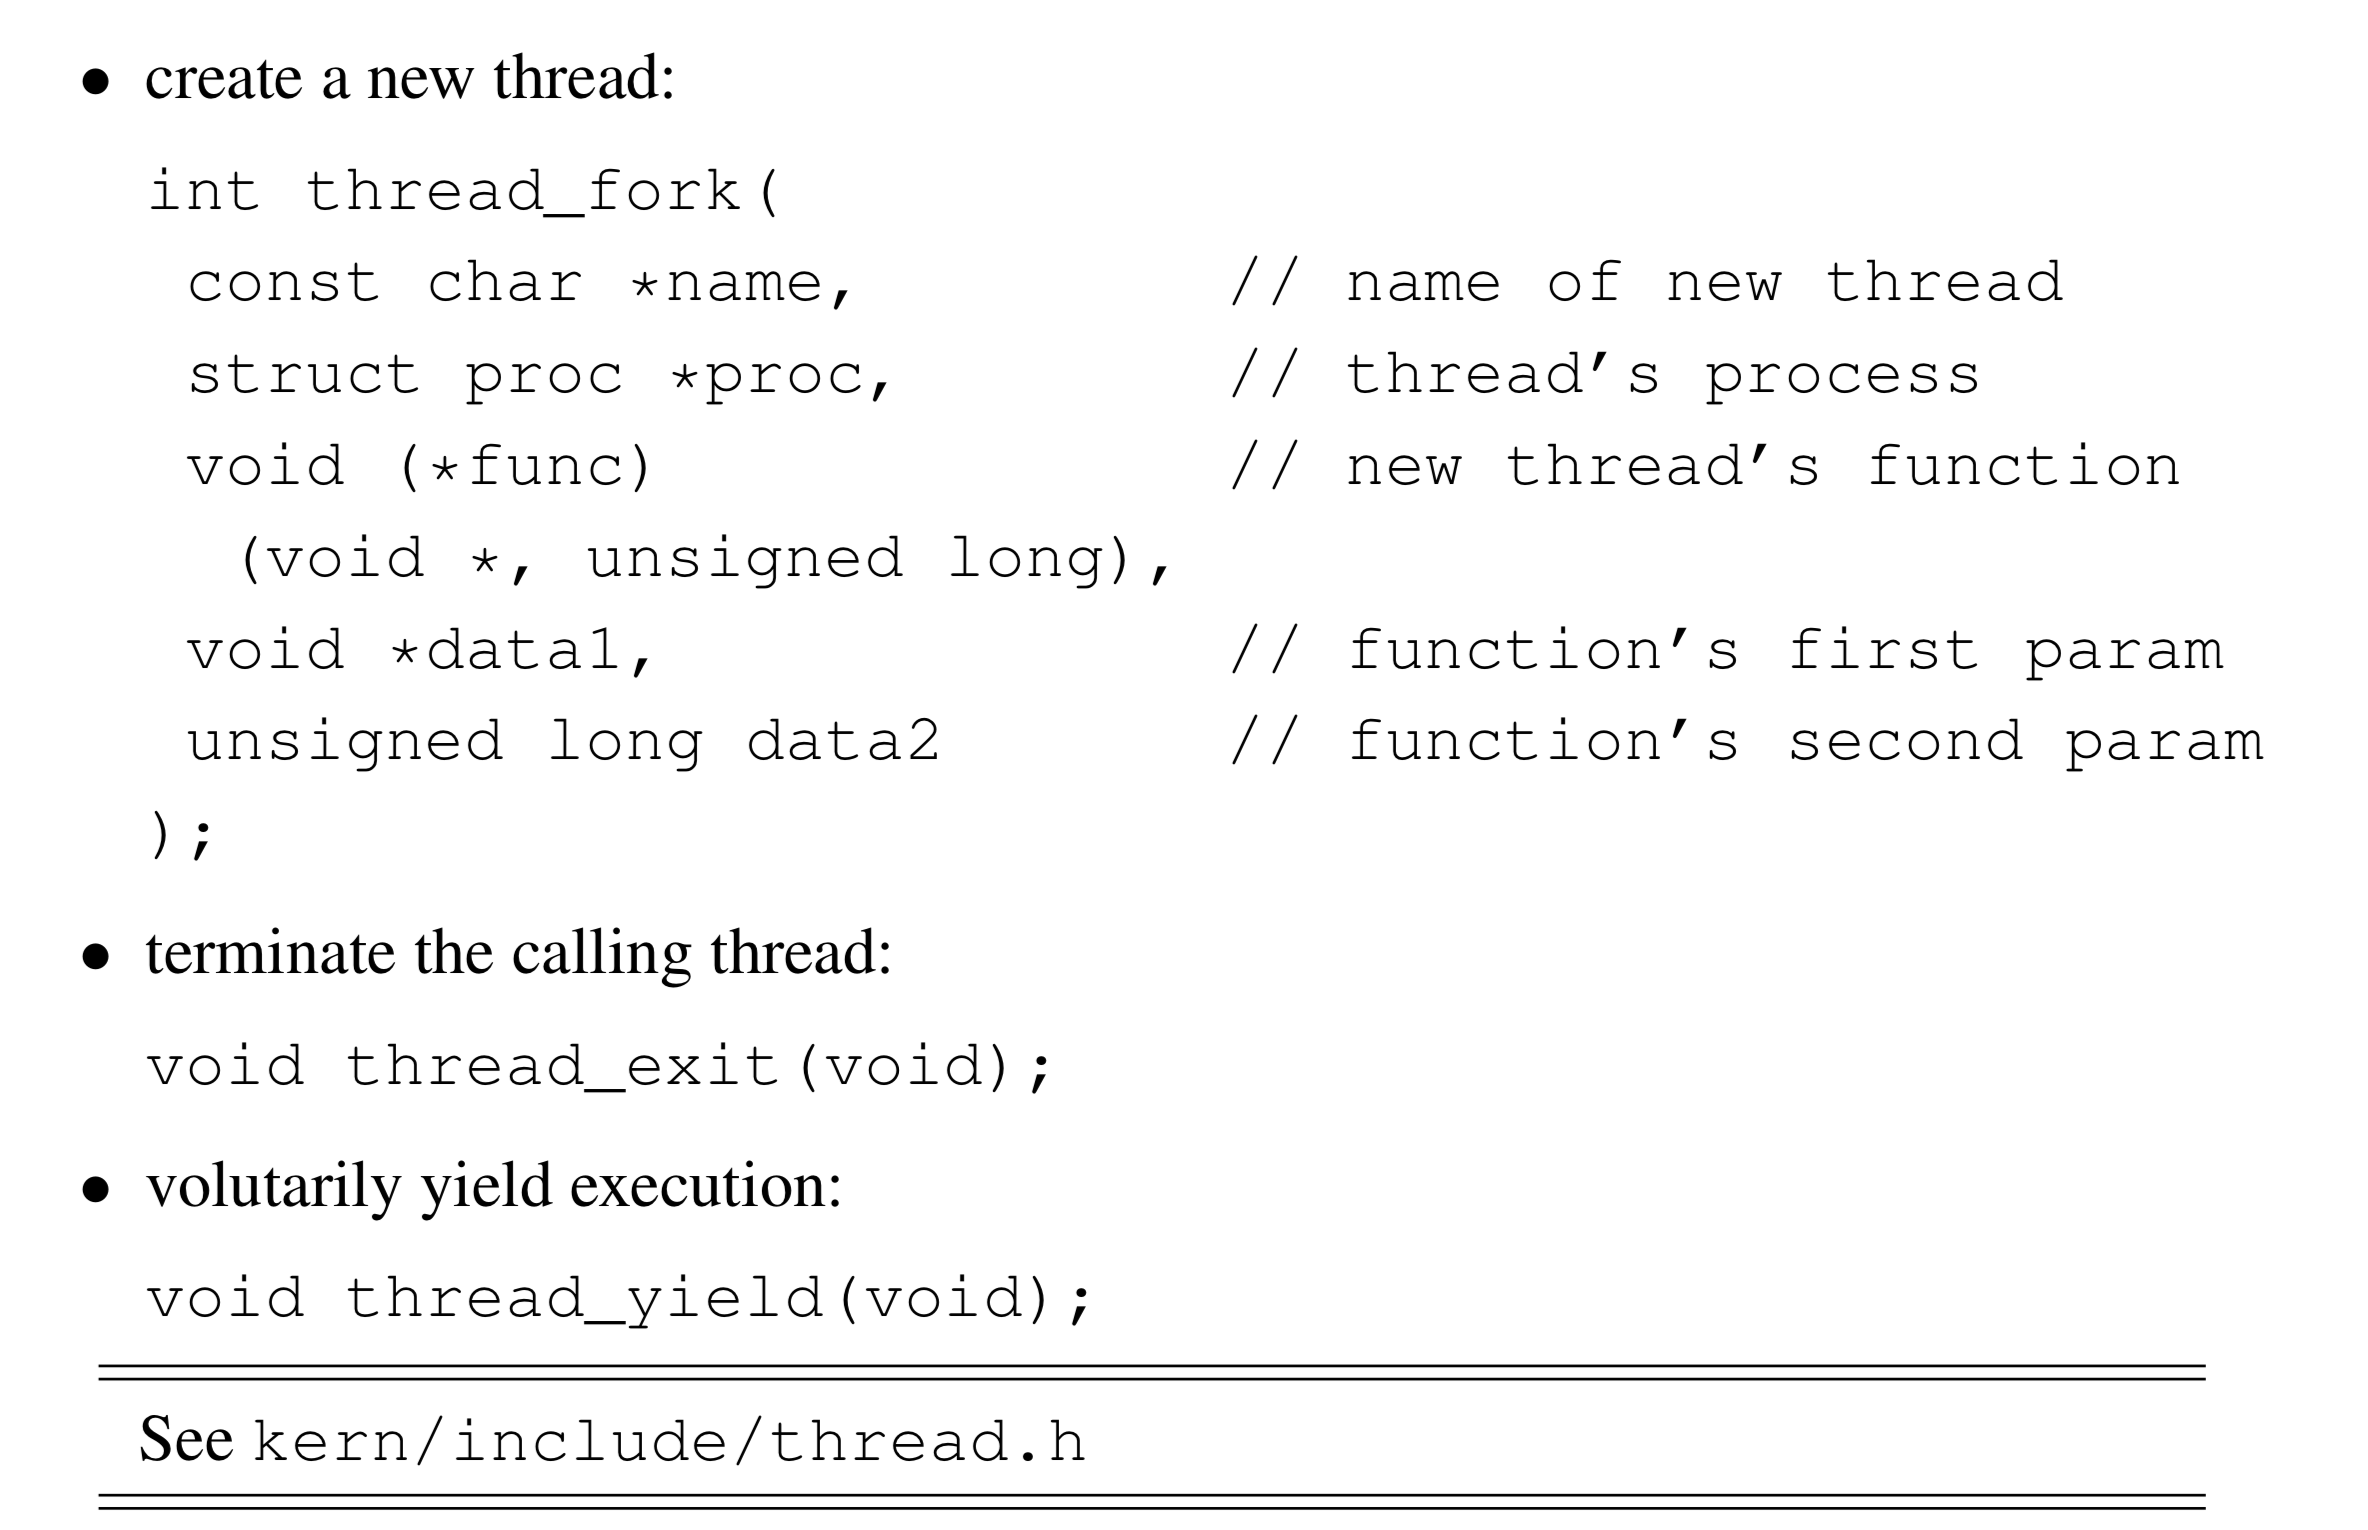
\includegraphics[scale=0.2]{1}\\
\textbf{Taken from lecture slides}
\end{center}
\newpage
\textbf{Why Threads?}

\begin{itemize}
\item parallelism exposed by threads enables parallel execution if the
underlying hardware supports it. – programs can run faster
\item parallelism exposed by threads enables better processor utilization 
\begin{itemize}
\item if one thread has to block, another may be able to run
\end{itemize} 
\end{itemize}
\end{document}





